\begin{pastexam}[label={px:ncku-108-ee-ds-04}]{成大電機所 108 學年度 問答題第 3 題}
（問答）

Given the following orders of traversal of a binary tree:

\quad\begin{tabular}{ll}
Postorder: & G, D, B, H, I, E, F, C, A\\
Inorder: & D, G, B, A, H, E, I, C, F\\
\end{tabular}

Is it possible to reconstruct the tree uniquely? If yes, reconstruct the tree and explain the
reason, otherwise justify your answer. (10 points)
\end{pastexam}

\begin{pastsoln}
\textbf{可以，而且唯一。} 節點的名字都不同時，後序加中序可以唯一決定一棵二元樹（和資結書定理~7.4
前序加中序的道理相同，資結書第~7.4~節）：
\begin{itemize}
\item 後序的\textbf{最後一個}一定是根。
\item 在中序裡找到根，根左邊的是左子樹的全部節點，右邊的是右子樹的全部節點，個數也就確定了。
\item 後序是「左子樹、右子樹、根」，所以後序扣掉最後的根之後，前面那幾個（個數等於左子樹的節點數）是
左子樹的後序，接著是右子樹的後序。
\item 對兩棵子樹遞迴做同樣的事。 每一步都只有一種切法，所以重建的結果唯一。
\end{itemize}

\textbf{重建}：
\begin{enumerate}
\item 後序最後是 A，根是 A。 中序 D G B $|$ A $|$ H E I C F：左子樹 $\{D, G, B\}$，右子樹 $\{H, E, I, C, F\}$。
後序拆成 G D B（左）、H I E F C（右）。
\item 左子樹：後序 G D B 的最後是 B，B 是 A 的左子節點。 中序 D G B：B 左邊是 D G，右邊空的。 子樹
$\{D, G\}$ 的後序 G D，根 D；中序 D G，D 的左邊空、右邊是 G。 所以 D 是 B 的左子節點，G 是 D 的
\textbf{右}子節點。
\item 右子樹：後序 H I E F C 的最後是 C，C 是 A 的右子節點。 中序 H E I $|$ C $|$ F：左子樹 $\{H, E, I\}$，
右子樹 $\{F\}$。 後序拆成 H I E、F。
\item $\{H, E, I\}$：後序最後是 E，中序 H E I，H 是 E 的左子節點、I 是右子節點。 F 是 C 的右子節點。
\end{enumerate}

\begin{center}
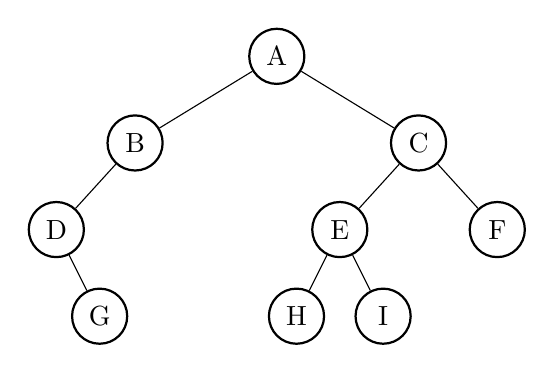
\begin{tikzpicture}[every node/.style={circle, draw, thick, minimum size=7mm, inner sep=0pt},
    level distance=11mm, level 1/.style={sibling distance=36mm}, level 2/.style={sibling distance=20mm},
    level 3/.style={sibling distance=11mm}]
\node {A}
  child {node {B}
    child {node {D}
      child[missing]
      child {node {G}}}
    child[missing]}
  child {node {C}
    child {node {E}
      child {node {H}}
      child {node {I}}}
    child {node {F}}};
\end{tikzpicture}
\end{center}

檢查：這棵樹的中序是 D G B A H E I C F，後序是 G D B H I E F C A，和題目相同。 （它的前序是
A B D G C E H I F。）

注意：如果給的是前序加後序，像 D 只有一個子節點 G 的情形，就分不出 G 在左還是在右，不一定唯一；一定要
有中序。
\end{pastsoln}
